\documentclass[11]{article}
\usepackage[margin=1in]{geometry}
\usepackage{amsfonts,amsmath,amssymb}
\usepackage{fancyhdr}
\usepackage{graphicx}
\usepackage{float}
\usepackage{transparent}
\usepackage{eso-pic}
\usepackage[colorlinks,linkcolor={blue}]{hyperref}



\usepackage{listings}
\usepackage{color}


\definecolor{dkgreen}{rgb}{0,0.6,0}
\definecolor{gray}{rgb}{0.5,0.5,0.5}
\definecolor{mauve}{rgb}{0.58,0,0.82}

\lstset{frame=tb,
  language=Java,
  aboveskip=3mm,
  belowskip=3mm,
  showstringspaces=false,
  columns=flexible,
  basicstyle={\small\ttfamily},
  numbers=none,
  numberstyle=\tiny\color{gray},
  keywordstyle=\color{blue},
  commentstyle=\color{dkgreen},
  stringstyle=\color{mauve},
  breaklines=true,
  breakatwhitespace=true,
  tabsize=3
}



\newcommand\BackgroundPic{%
\put(0,0){%
\parbox[b][\paperheight]{\paperwidth}{%
\vfill
\centering
{\transparent{0.3} 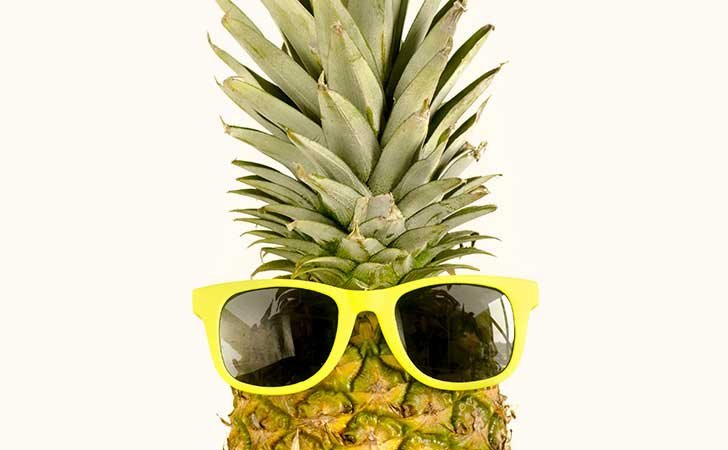
\includegraphics[width=\paperwidth,height=\paperheight,%
keepaspectratio]{background.jpg}}%
\vfill
}}}

\AddToShipoutPicture*{\BackgroundPic}

\pagestyle{fancy}
\fancyhead{}
\fancyfoot{}
\fancyhead[L]{\slshape \MakeUppercase{Notes}}
\fancyfoot[C]{\thepage}
%\renewcommand{\headrulewidth}{0pt}
\renewcommand{\footrulewidth}{0pt}

\parindent 0ex
\renewcommand{\baselinestretch}{1.5}

\begin{document}
\begin{titlepage}
\begin{center}
\vspace{1cm}
\Large{\textbf{Computer Science 101: Introduction to Java and Algorithms}}\\
\vfill
\line(1,0){400}\\
\huge{\textbf{Section 4: Arrays}}\\
\line(1,0){400}\\
\vfill
Erudition Labs\\
Computer Science 101: Introduction to Java and Algorithms\\
\today\\
\end{center}
\end{titlepage}

\tableofcontents
\thispagestyle{empty}
\clearpage
\setcounter{page}{1}

\section{Terminology}
\begin{itemize}
  \item \textbf{\textit{Memory}} --
  Memory is where all the action happens. Many people often refer to it as storage space although that is not entirely true. When programmers talk of memory, we are talking about addressable memory. This means memory that computers can create addresses for and thus use. Memory is NOT hard drive space. It is RAM. The amount of memory you have depends on two things. The amount of RAM you have and the operating systems you are using (eg. 32 bit windows vs 64 bit windows). With 32 bit systems, you are limited to 4 GB of ram where as 64 bit machines are (theoretically since we haven`t done it) limited to 16.8 million terabytes of RAM. Everything happens in your memory. When you start up your computer, windows (or mac, linux, android, IOS...whatever) gets loaded into memory. Whenever you launch a program, it gets loaded into memory. Pretty much whenever you do anything on a computer, it`s done in memory. As a programmer, you generally deal with two types of memory, heap and stack. Refer to \autoref{sec:heap} to lean more about heap vs stack.

  

\end{itemize}
\section{Pre-Chapter}


\end{document}